
%(BEGIN_QUESTION)
% Copyright 2011, Tony R. Kuphaldt, released under the Creative Commons Attribution License (v 1.0)
% This means you may do almost anything with this work of mine, so long as you give me proper credit

Examine this ladder logic program for an Allen-Bradley MicroLogix PLC controlling a motor, with multiple ``Start,'' ``Stop,'' and safety pull-switch shutdowns:

$$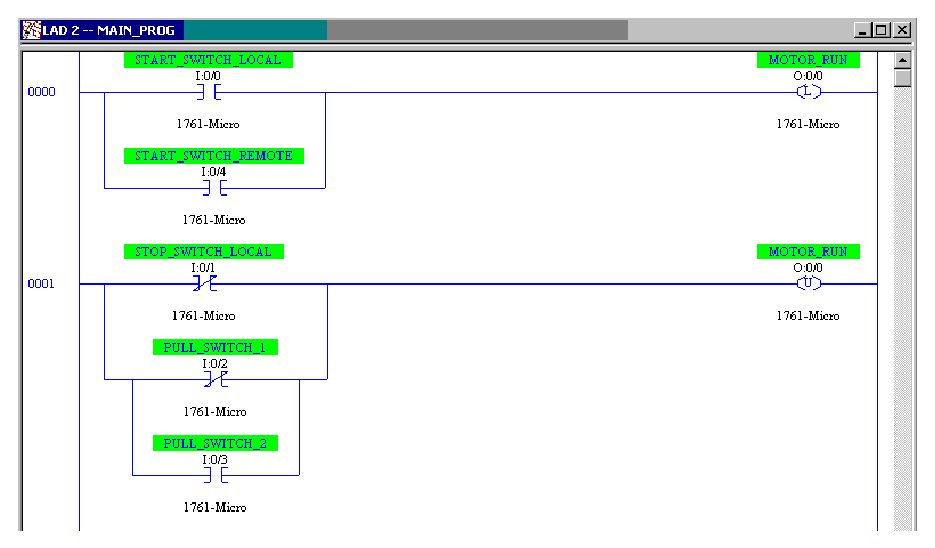
\includegraphics[width=15.5cm]{i03854x01.eps}$$

Based on this program, determine the necessary type of hard-wired switch contact for each input switch:

\begin{itemize}
\item{} {\tt START\_SWITCH\_LOCAL}: {\it normally-open} (NO) or {\it normally-closed} (NC)?
\vskip 5pt
\item{} {\tt START\_SWITCH\_REMOTE}: {\it normally-open} (NO) or {\it normally-closed} (NC)?
\vskip 5pt
\item{} {\tt STOP\_SWITCH\_LOCAL}: {\it normally-open} (NO) or {\it normally-closed} (NC)?
\vskip 5pt
\item{} {\tt PULL\_SWITCH\_1}: {\it normally-open} (NO) or {\it normally-closed} (NC)?
\vskip 5pt
\item{} {\tt PULL\_SWITCH\_2}: {\it normally-open} (NO) or {\it normally-closed} (NC)?
\end{itemize}

Also, identify at least two different faults independently capable of preventing the motor from starting up despite attempts actuating the local start switch {\it and} actuating the remote start switch:

\vskip 10pt

\begin{itemize}
\item{} 
\vskip 20pt
\item{} 
\end{itemize}

\vfil
\underbar{file i03854}
\eject
%(END_QUESTION)





%(BEGIN_ANSWER)

This is a graded question -- no answers or hints given!

%(END_ANSWER)





%(BEGIN_NOTES)

This happens to be one of those unusual cases where the type of real-world switch contact exactly matches its virtual switch contact instruction inside the PLC in every case.  Since this program uses retentive coil instructions (``Latch'' and ``Unlatch'') which require virtual power in order to take action, we desire each of these switches to send virtual power to the respective coil when actuated.  When one of the normally-open (NO) switches is actuated, it sends real power to the PLC input channel, setting the input register bit (1), causing the NO contact instruction to close and send virtual power to the coil.  When one of the normally-closed (NC) switches is actuated, it halts real power from getting to the PLC input, clearing the input register bit (0), causing the NC contact instruction to close and send virtual power to the coil.  Therefore:

\begin{itemize}
\item{} {\tt START\_SWITCH\_LOCAL}: {\bf normally-open} (NO)
\item{} {\tt START\_SWITCH\_REMOTE}: {\bf normally-open} (NO)
\item{} {\tt STOP\_SWITCH\_LOCAL}: {\bf normally-closed} (NC)
\item{} {\tt PULL\_SWITCH\_1}: {\bf normally-closed} (NC)
\item{} {\tt PULL\_SWITCH\_2}: {\bf normally-open} (NO)
\end{itemize}

\vskip 10pt

\noindent
Some possible faults causing motor to not start from either start switch:

\begin{itemize}
\item{} Open fault in local start switch wiring
\item{} Open fault in remote start switch wiring
\item{} Open fault in local stop switch wiring
\item{} Open fault in pull switch \#1 wiring
\item{} Shorted fault (sending power to PLC input at all times) in pull switch \#2 wiring
\item{} Open fault in motor contactor circuit
\item{} PLC program execution halted (e.g. not in Run mode)
\end{itemize}


%INDEX% PLC, ladder logic programming: determining necessary switch types from program

%(END_NOTES)


